\documentclass{ctexart}
\usepackage{tabularx}
\usepackage{float}
\usepackage{pdfpages}
\usepackage{graphicx}
\usepackage{geometry}
\title{听觉文化与世界文明期末考试}
\author{陈启钰}
\date{\today}
\begin{document}
	\maketitle
	\section{必答表格题}
	\begin{figure}[H]
		\centering
		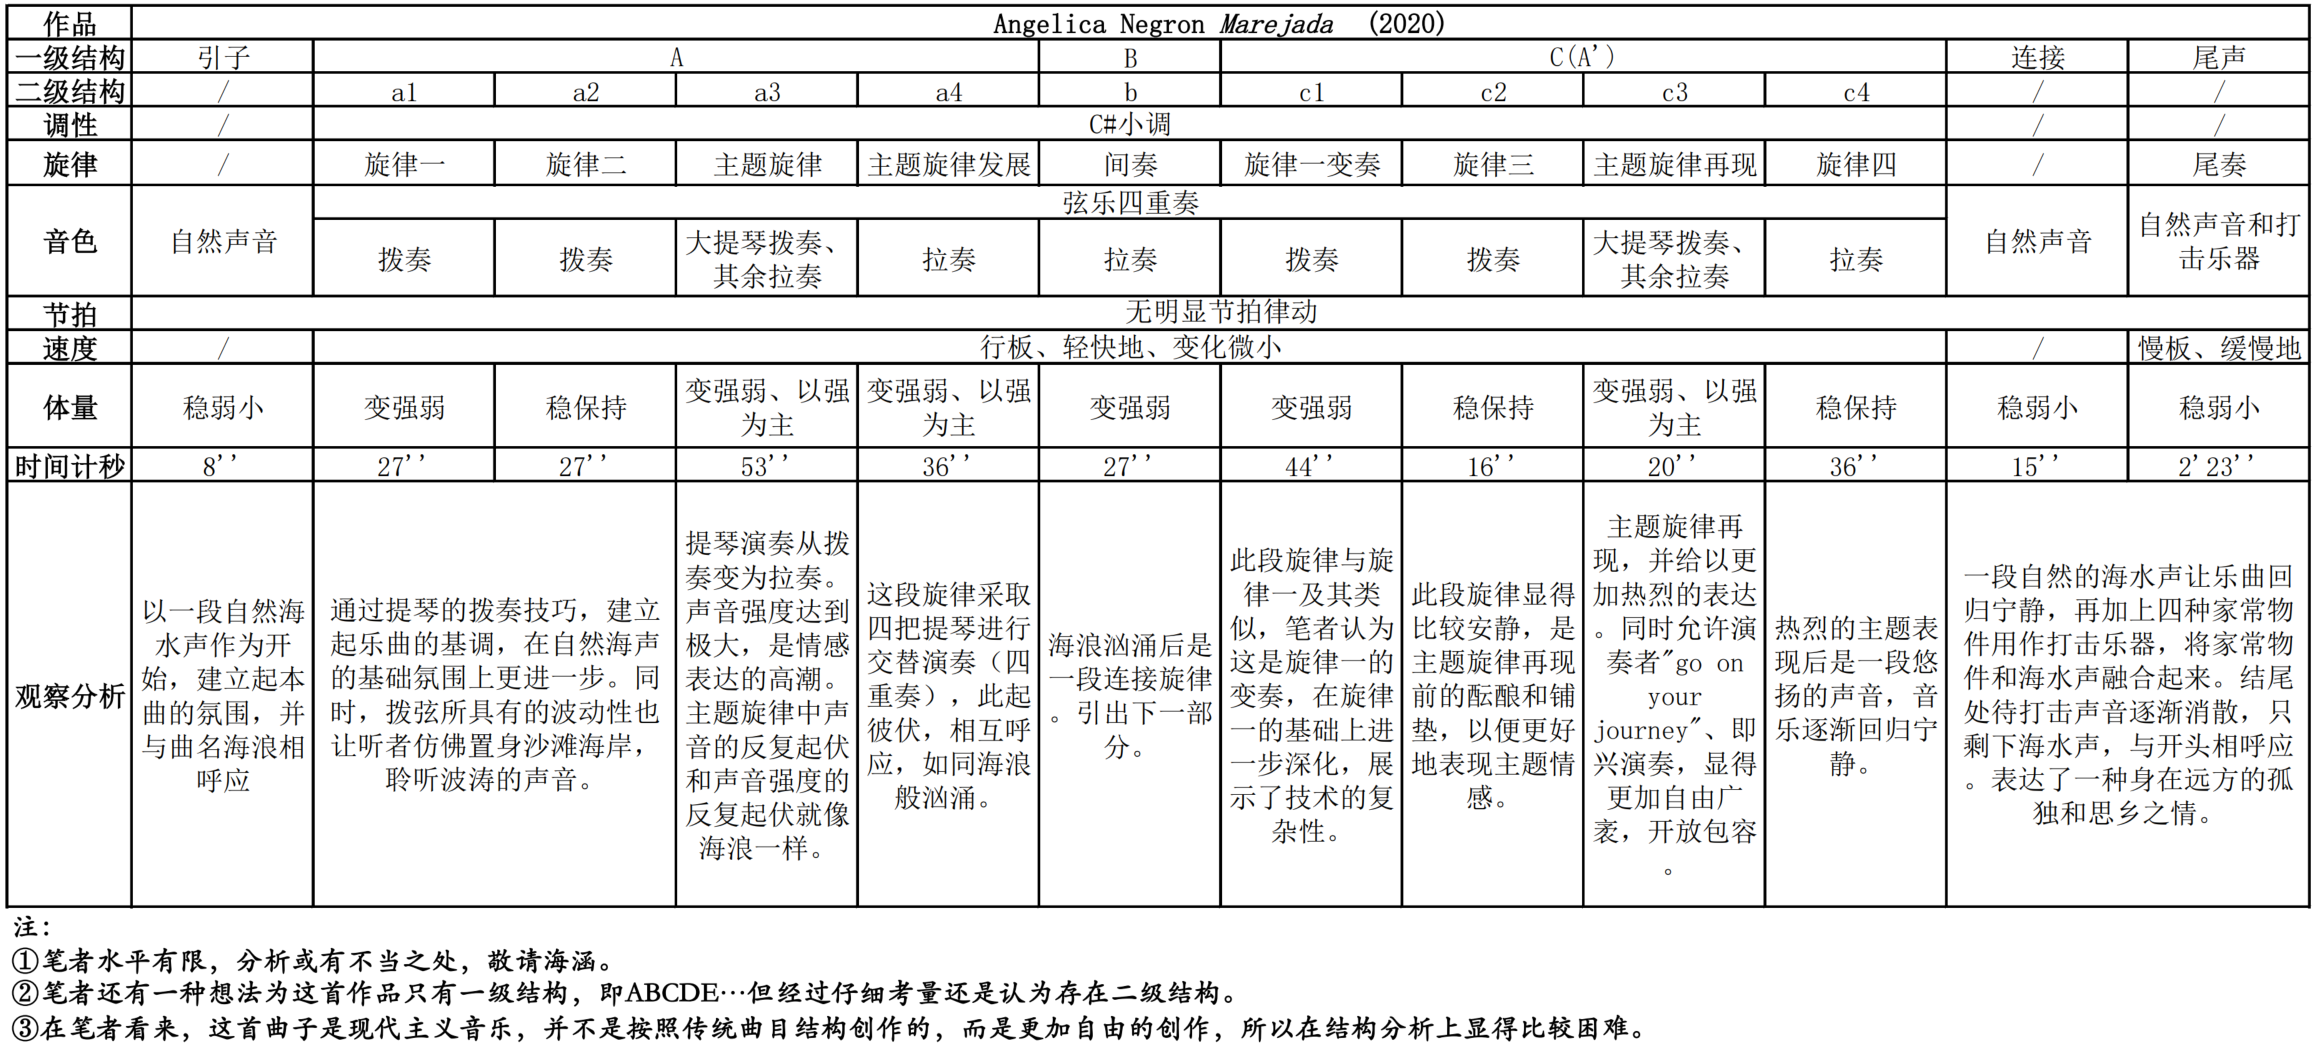
\includegraphics[width=\linewidth]{marejada.png}
	\end{figure}
	\section{必答辨析题}
	\subsection{《贝七二乐章》和《葬礼进行曲》比较}
	作品方案:《贝七二乐章》和《葬礼进行曲》都是葬礼进行曲,两者都表达了对阵亡将士的缅怀和对受伤士兵的抚慰。两者的不同之处在于,《贝七二乐章》虽然忧郁,但哀而不伤,不仅有送葬的忧思之情,还有着一丝乐观、朝气蓬勃的力量;《葬礼进行曲》相比则更加悲壮宏伟。
	
	声音方案:两首乐曲中,中提琴和大提琴组成的低声部都营造了安静的氛围。同时,两首乐曲都重复多次各自的主旋律。不同之处在于,《贝七二乐章》速度稍快,且具有节奏感,旋律更加优美,整体听觉更加柔和,单簧管、长笛、小提琴等乐器为乐曲增添了明朗的色彩;《葬礼进行曲》速度稍慢,节奏感不明显,旋律要凄凉一些,铜管乐器的更多应用为乐曲增添悲壮色彩和宏伟的感受。
	\subsection{《乘风破浪》、《蓝色多瑙河》与《皇帝》}
	《乘风破浪》风格更接近《蓝色多瑙河》。
	
	三首乐曲都是圆舞曲,均以稳定为主,服从舞曲功能要求。不同的是,《乘风破浪》和《蓝色多瑙河》更加优美流畅、舒缓愉快,而《皇帝》的旋律更加庄重雄伟,有皇家气质。音色方面,《乘风破浪》和《蓝色多瑙河》以温和的弦乐和木管居多,而《皇帝》中有更多雄壮恢弘的铜管乐器。节奏方面,《皇帝》进行曲和圆舞曲律动感并置,而《乘风破浪》和《蓝色多瑙河》无进行曲的律动感。结构方面,《乘风破浪》和《蓝色多瑙河》由多个独立的圆舞曲段落构成,最后合并成一个整体,而《皇帝》在圆舞曲连缀基础上安置了一个进行曲作为开头,在三拍子舞蹈律动中融入了进行曲,将进行曲仪式感和圆舞曲娱乐干混融。
	
	\subsection{对《海浪》的个人体验}
	初听《海浪》时,笔者因为乐曲缺乏优美的主旋律而十分困惑,乐曲高潮部分的“嘈杂混乱”尤甚,很难称之“好听”。多次聆听《海浪》后,笔者才明白这首曲子并不是传统音乐,所以不具有传统的音乐结构等。传统音乐具有核心聆听方向,即伴奏声部和核心声部明显(或声部合并),使得听者能够轻易把控。《海浪》应属于现代主义音乐范畴,不再拘泥于传统,它的节奏更加自由,没有固定拍子,乐器表达更加自由。同时,现代主义音乐的聆听方向是分散的,导致听觉导向缺失。笔者明白这一点后,又反复听了多次,逐渐理解创作者的手法,领会创作者想表达的情感。这说明,是否喜欢一首音乐不是个人的原因,而是作曲家和听者共谋的结果,即我们应该折中聆听。
\end{document}